\textbf{Magic123}~--~Magic123 employs a unique approach that integrates both 2D and 3D priors for generating 3D objects. The method initiates by processing an input image, creating multiple perspectives of the intended object. The input image, depicted in Figure~\ref{fig:inputAndModel} part (b), was generated using the same prompt with Dall-E 3. The initial phase involves constructing a low-quality, coarse model complete with texture, forming a basic representation of the object. Subsequently, this model undergoes a refinement stage, where additional details are added to both the object and its texture.

\begin{figure}[H]
    \centering
    % Subfigure for textual description
    \begin{subfigure}[b]{0.25\textwidth}
        \centering
        \fontsize{9pt}{7pt}\selectfont\text{Iteration = 100}\vspace{.1cm}
        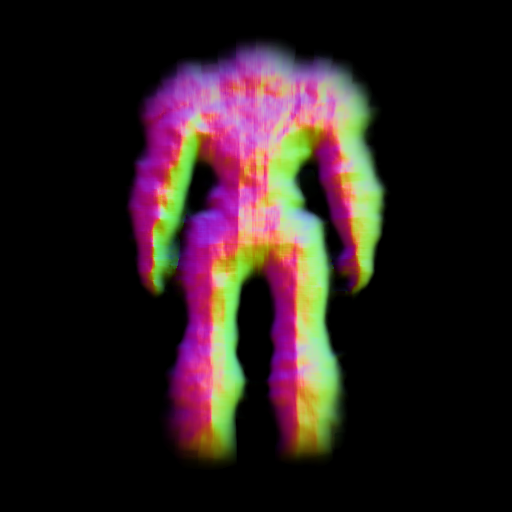
\includegraphics[width=\textwidth]{etc/a robot made out of plants/magic123/magic123_coarse_robot_front_0_part2.png}
        
\includegraphics[width=\textwidth]{etc/a robot made out of plants/magic123/magic123_coarse_robot_front_0_part1.png}
        \caption{}
    \end{subfigure}
    \begin{subfigure}[b]{0.25\textwidth}
        \centering
        \fontsize{9pt}{7pt}\selectfont\text{Iteration = 5000}\vspace{.1cm}
        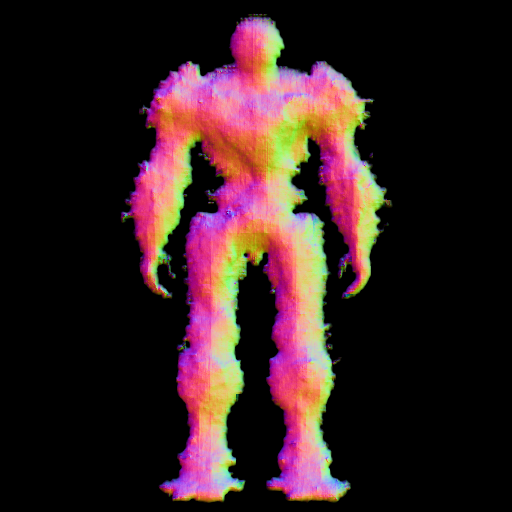
\includegraphics[width=\textwidth]{etc/a robot made out of plants/magic123/magic123_coarse_robot_front_5000_part2.png}
        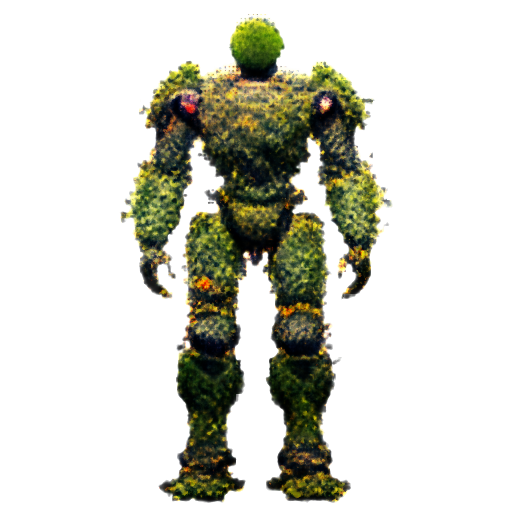
\includegraphics[width=\textwidth]{etc/a robot made out of plants/magic123/magic123_coarse_robot_front_5000_part1.png}
        \caption{}
    \end{subfigure}
    \begin{subfigure}[b]{0.25\textwidth}
        \centering
        \fontsize{9pt}{7pt}\selectfont\text{Iteration = 10000}\vspace{.1cm}
        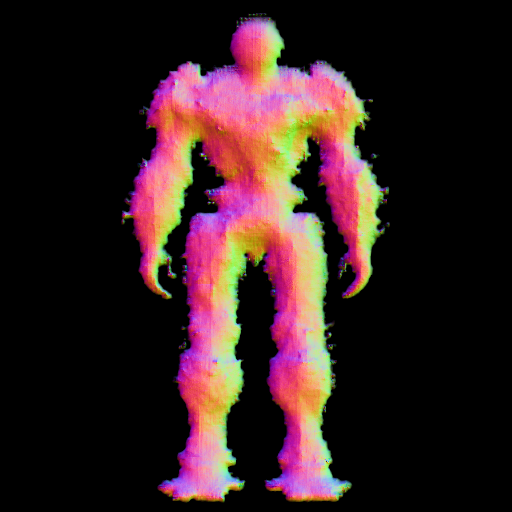
\includegraphics[width=\textwidth]{etc/a robot made out of plants/magic123/magic123_coarse_robot_front_10000_part2.png}
        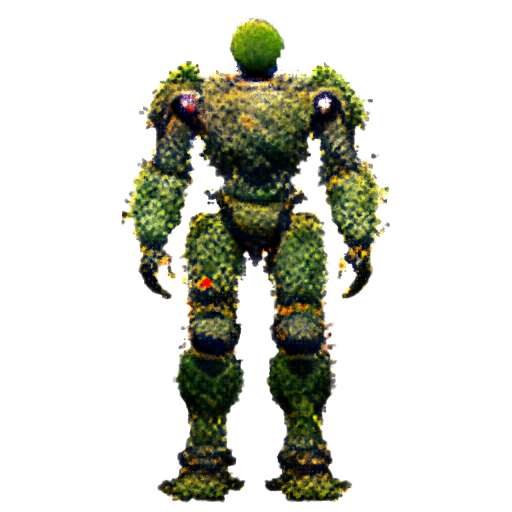
\includegraphics[width=\textwidth]{etc/a robot made out of plants/magic123/magic123_coarse_robot_front_10000_part1.png}
        \caption{}
    \end{subfigure}
    \caption{Front view of the coarse stage of Magic123}~\label{fig:generationFrontCoarseMagic123}
\end{figure}

The front view of the coarse generation process is depicted in Figure~\ref{fig:generationFrontCoarseMagic123}. Even at an early stage like Iteration 100, the method efficiently produces an outline that resonates well with the input image, including the incorporation of a green hue to represent the plant aspects. Progressing to Iteration 5000, the model becomes more detailed, with sharper edges and a more defined robotic shape. Elements suggestive of overgrowth, such as leaves and vines, begin to emerge, and the texture convincingly integrates plant-like features, covering the model with grass and vine patterns. By Iteration 10000 in this stage, the model's shape does not evolve significantly, but some color variation in the plant textures and distinct features like a white spot on the right shoulder and a bright red dot above the left knee emerge, hinting at metallic robot parts and a blooming flower, respectively.

During the refinement stage, showcased in Figure~\ref{fig:generationFrontRefineMagic123}, the model initially loses some of its detailed and mossy character from the coarse stage. Floating parts disconnected from the main body become noticeable, particularly on the right arm and the left leg. Compared to the 10000th iteration of the coarse stage, the texture seems less detailed initially. However, by Iteration 5000, the texture regains and even surpasses its former level of detail, presenting a more realistic plant-like structure. The model appears covered in grass, moss, and vines, with enhanced features like a more pronounced blooming flower and more defined hands, knees, shoulders, and feet. Further into Iteration 10000, the model becomes smoother, particularly around the thighs and chest, though the floating parts persist. The texture at this stage is remarkably detailed, offering a realistic plant appearance with effective light and shadow interplay, particularly around the stomach area.

\begin{figure}[H]
    \centering
    % Subfigure for textual description
    \begin{subfigure}[b]{0.25\textwidth}
        \centering
        \fontsize{9pt}{7pt}\selectfont\text{Iteration = 100}\vspace{.1cm}
        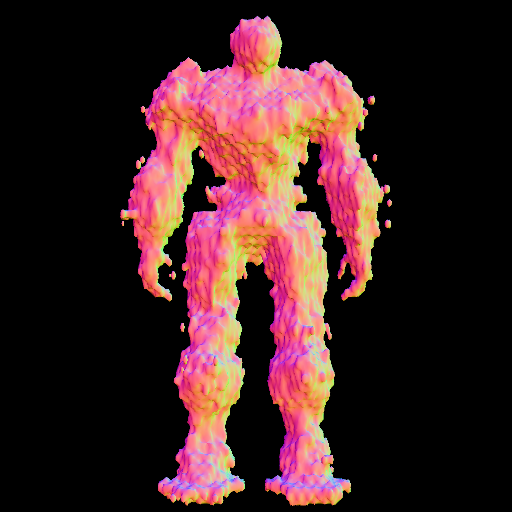
\includegraphics[width=\textwidth]{etc/a robot made out of plants/magic123/magic123_refine_robot_front_0_part2.png}
        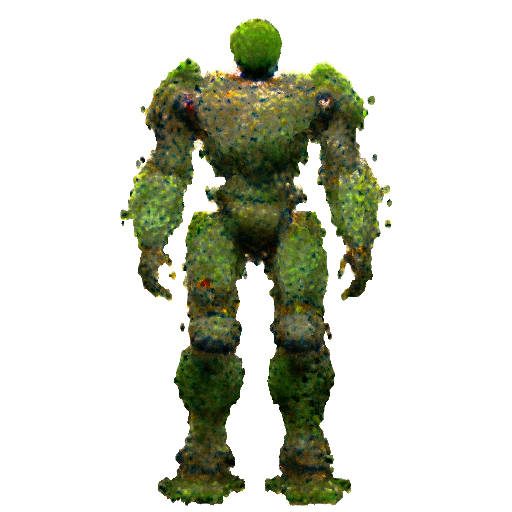
\includegraphics[width=\textwidth]{etc/a robot made out of plants/magic123/magic123_refine_robot_front_0_part1.png}
        \caption{}
    \end{subfigure}
    \begin{subfigure}[b]{0.25\textwidth}
        \centering
        \fontsize{9pt}{7pt}\selectfont\text{Iteration = 5000}\vspace{.1cm}
        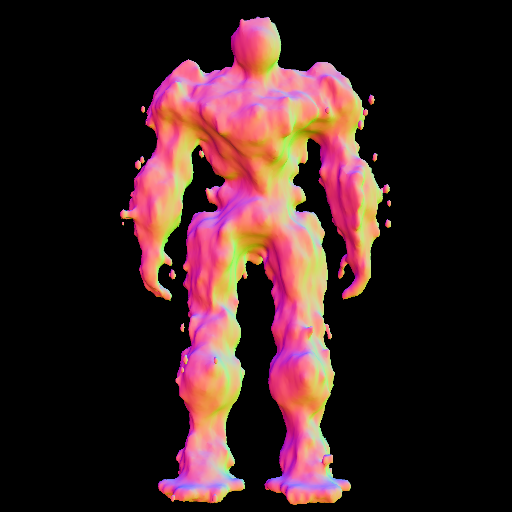
\includegraphics[width=\textwidth]{etc/a robot made out of plants/magic123/magic123_refine_robot_front_5000_part2.png}
        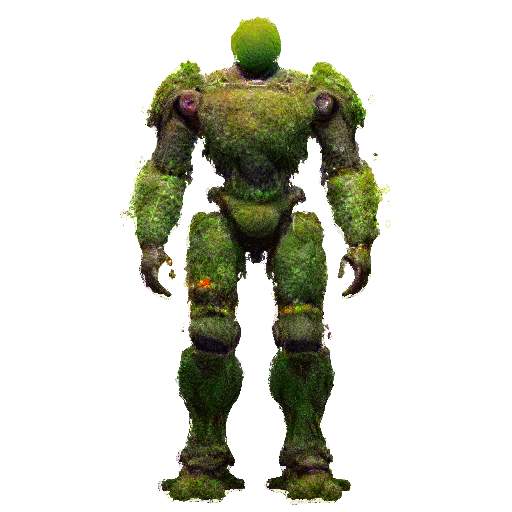
\includegraphics[width=\textwidth]{etc/a robot made out of plants/magic123/magic123_refine_robot_front_5000_part1.png}
        \caption{}
    \end{subfigure}
    \begin{subfigure}[b]{0.25\textwidth}
        \centering
        \fontsize{9pt}{7pt}\selectfont\text{Iteration = 10000}\vspace{.1cm}
        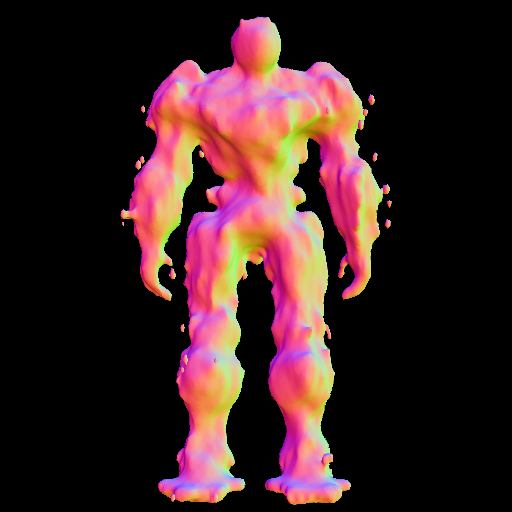
\includegraphics[width=\textwidth]{etc/a robot made out of plants/magic123/magic123_refine_robot_front_10000_part2.png}
        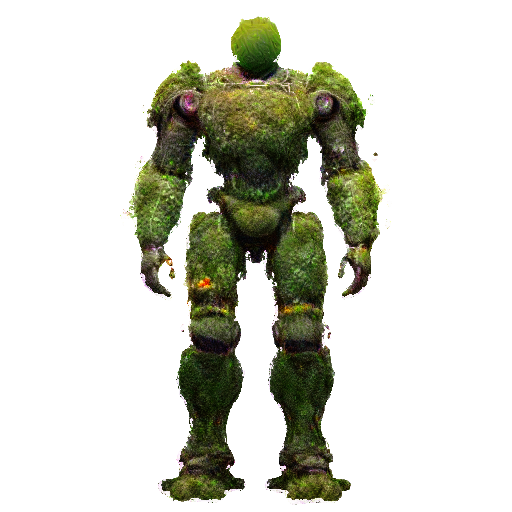
\includegraphics[width=\textwidth]{etc/a robot made out of plants/magic123/magic123_refine_robot_front_10000_part1.png}
        \caption{}
    \end{subfigure}
    \caption{Front view of the refine stage of Magic123}~\label{fig:generationFrontRefineMagic123}
\end{figure}

As Magic123 generates multiple views during training, additional perspectives of the object for each iteration can be seen in Figures~\ref{fig:generationCoarseMagic123} and~\ref{fig:generationRefineMagic123} in the appendix, which include the right, back, and left views. In there one can see the difficulties magic123 had in the beginning while determining the side views of the model. These problems however quickly dissapeared until Iteration 5000. 

The final mesh, as illustrated in part (a) of Figure~\ref{fig:inputAndModel}, exhibits reasonable quality. Some white spots, particularly around the floating parts, suggest that these areas may remain textureless due to rendering issues. In comparison, the final model does a commendable job in mirroring the overall shape of the input image. Despite this, it becomes evident that Magic123 struggles to replicate the complex details of the plants. This shortcoming highlights the limitations of the method when it comes to fully capturing and translating the details in the input image into the 3D model. However, longer training iterations and higher computing power could mitigate this.

\begin{figure}[H]
    \centering
    \begin{subfigure}[b]{0.23\textwidth}
        \centering
        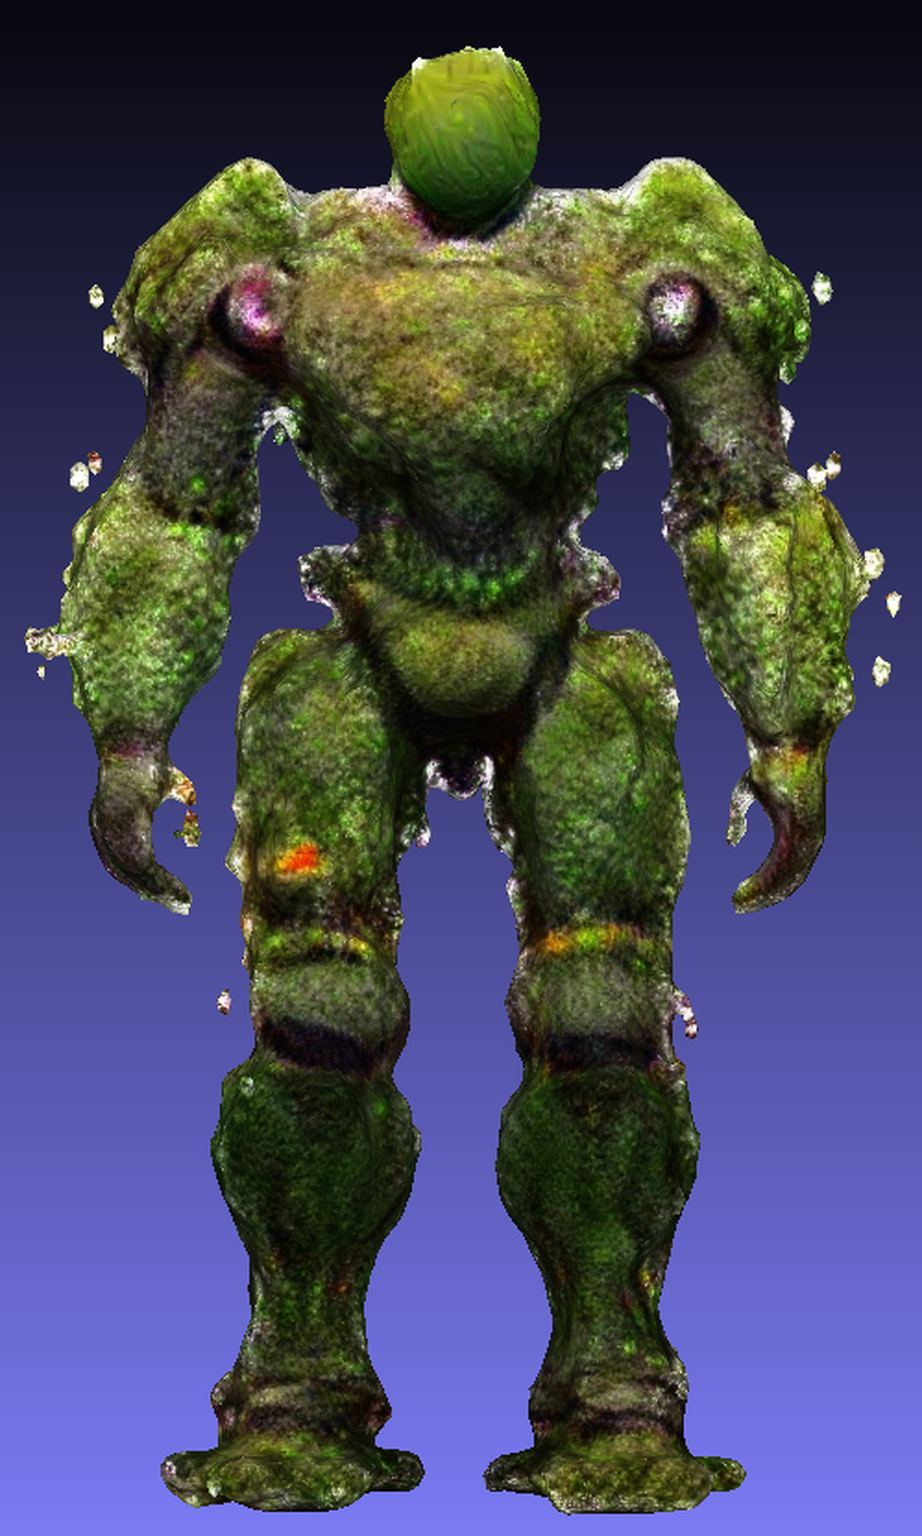
\includegraphics[width=\textwidth]{etc/a robot made out of plants/magic123/magic123_plantRobot_model_resized.png}
        \caption{Magic123}
    \end{subfigure}
    \begin{subfigure}[b]{0.38\textwidth}
        \centering
        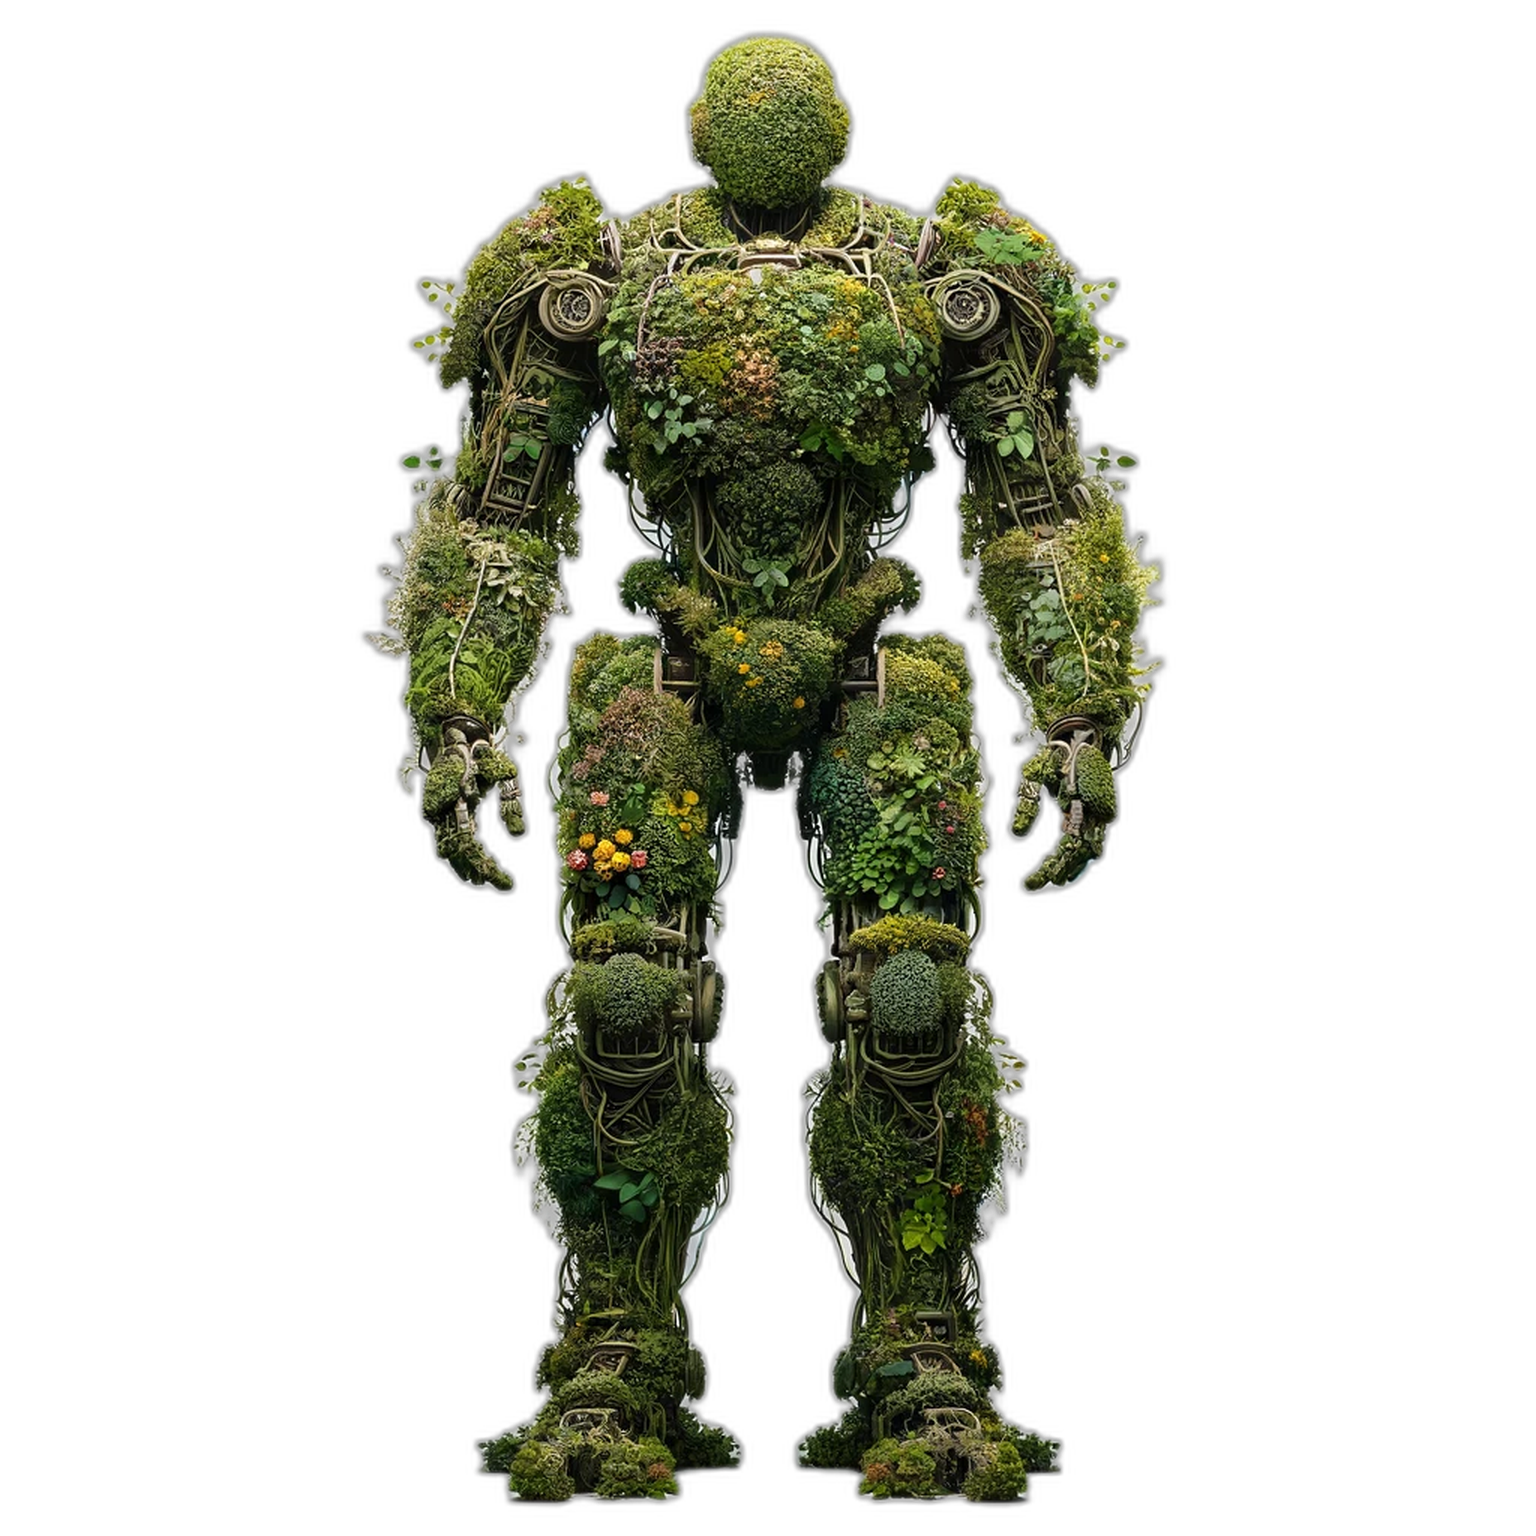
\includegraphics[width=\textwidth]{etc/a robot made out of plants/magic123/robot made out of plants_noBG_resized.png}
        \caption{Input Image}
    \end{subfigure}
    \begin{subfigure}[b]{0.21\textwidth}
        \centering
        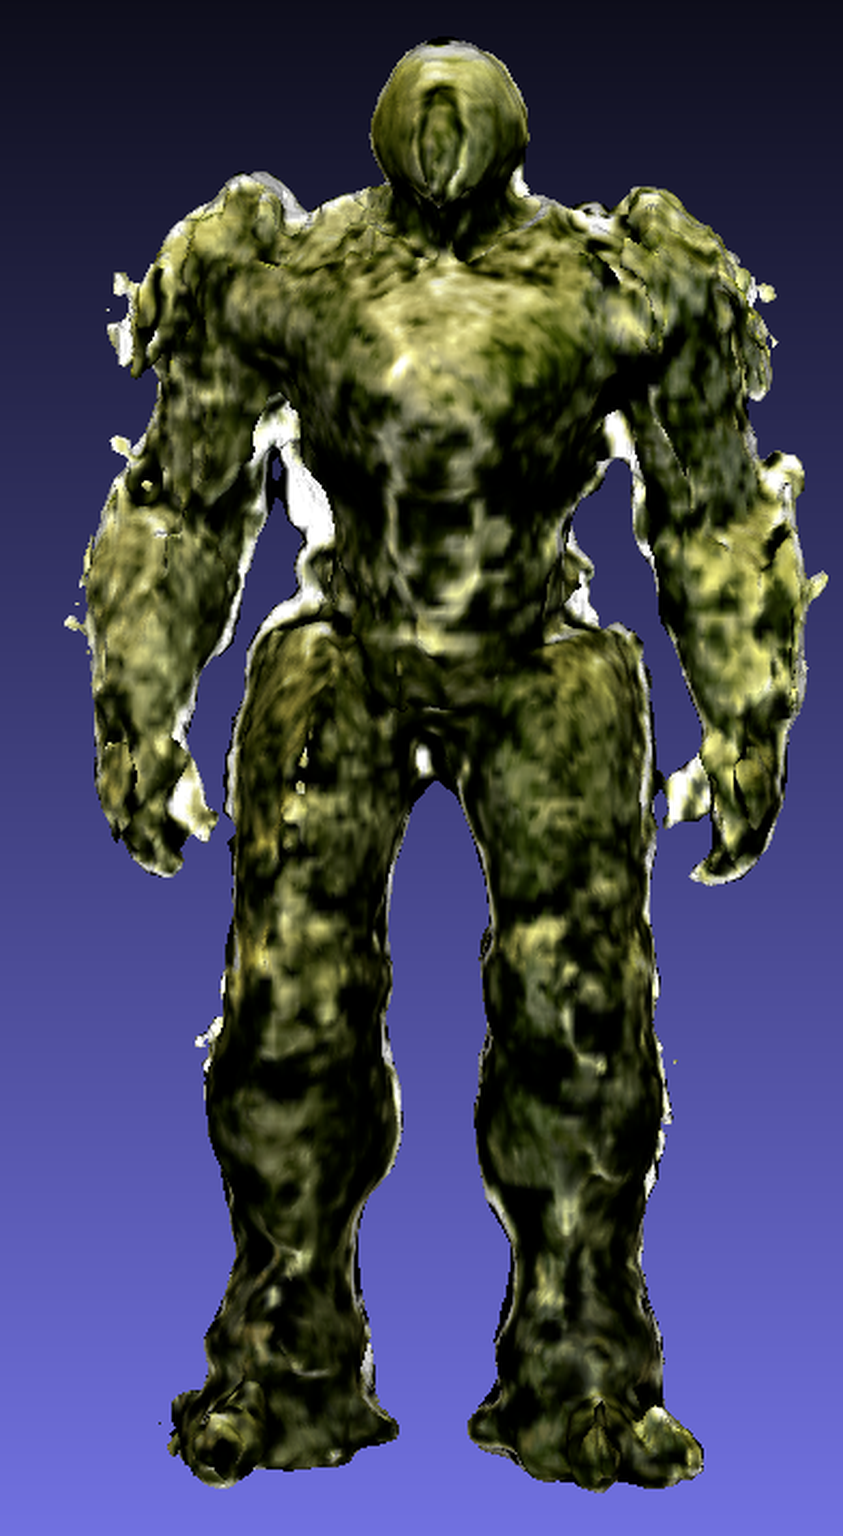
\includegraphics[width=\textwidth]{etc/a robot made out of plants/wonder3d/wonder3d_plantrobot_model_resized}
        \caption{Wonder3D}
    \end{subfigure}
    \caption{3D models generated by Magic123 and Wonder3D based on an imput image}~\label{fig:inputAndModel}
  \end{figure}